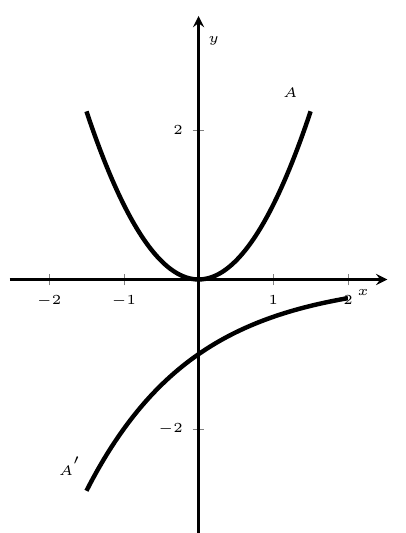
\begin{tikzpicture}
\begin{axis}[ 
xlabel=$x$,
ylabel=$y$,
axis x line=center, xlabel style={anchor=north west},
axis y line=center, ylabel style={anchor=south west},
xmin=-2,
xmax=2,
ymin=-3,
ymax=3,
axis line style={thick, shorten > = -0.5cm, shorten < = -0.5cm},
samples=50,
unit vector ratio*=1 1,
font=\tiny
]



\addplot [domain=-1.5:1.5, ultra thick, black, smooth]{x*x};
\addplot [domain=-1.5:2, ultra thick, black, smooth]{-2^(-x)};

\node[right] at (axis cs:1.,2.5) {$A$};
\node[right] at (axis cs:-2.,-2.5) {$A^{'}$};
\end{axis};
\end{tikzpicture}